\documentclass[letterpaper,11pt]{article}
\oddsidemargin -1.0cm \textwidth 17.5cm

\usepackage[utf8]{inputenc}
\usepackage[activeacute,spanish, es-lcroman]{babel}
\decimalpoint
\usepackage{amsfonts,setspace}
\usepackage{amsmath}
\usepackage{amssymb, amsmath, amsthm}
\usepackage{comment}
\usepackage{float}
\usepackage{amssymb}
\usepackage{dsfont}
\usepackage{anysize}
\usepackage{multicol}
\usepackage{enumerate}
\usepackage{graphicx}
\usepackage[left=1.5cm,top=2cm,right=1.5cm, bottom=1.7cm]{geometry}
\setlength\headheight{1.5em} 
\usepackage{fancyhdr}
\usepackage{multicol}
\usepackage{hyperref}
\usepackage{wrapfig}
\usepackage{subcaption}
\usepackage{siunitx}
\usepackage{cancel}
\usepackage{mdwlist}
\usepackage{svg}
\pagestyle{fancy}
\fancyhf{}
\renewcommand{\labelenumi}{\normalsize\bfseries P\arabic{enumi}.}
\renewcommand{\labelenumii}{\normalsize\bfseries (\alph{enumii})}
\renewcommand{\labelenumiii}{\normalsize\bfseries \roman{enumiii})}


\begin{document}

\fancyhead[L]{\itshape{Facultad de Ciencias F\'isicas y Matem\'aticas}}
\fancyhead[R]{\itshape{Universidad de Chile}}

\begin{minipage}{11.5cm}
    \begin{flushleft}
        \hspace*{-0.6cm}\textbf{FI1000-1 Introducción a la Física Clásica}\\
        \hspace*{-0.6cm}\textbf{Profesora:} Paulina Lira\\
        \hspace*{-0.6cm}\textbf{Auxiliares:} Alejandro Cartes \& Juan Cristóbal Castro\\
        \hspace*{-0.6cm}\textbf{Ayudantes:} Francisca Bórquez \& Catalina Molina\\
    \end{flushleft}
\end{minipage}

\begin{picture}(2,3)
    \put(366, 10){
\includegraphics[scale=0.9]{2020-1/Imágenes/logo/dfi-fcfm.pdf}}
\end{picture}

\begin{center}
	\LARGE\textbf{Auxiliar Extra Crec2}\\
	\Large{Hidrostática + repaso}
\end{center}

\vspace{-1cm}
\begin{enumerate}\setlength{\itemsep}{0.4cm}

\rfoot[]{pág. \thepage}

\item[]

\item Considere las situaciones a) y b) de la Fig. 1, ambas en equilibrio. En el caso a) una esfera de radio y densidad desconocidas se encuentra sujeta a una masa $m_1$. En b) la misma esfera se encuentra totalmente sumergida en agua y conectada a una masa $m_2$. En ambos casos las cuerdas y poleas son ideales.   
\vspace{0.05cm}  
    
Calcule el radio de la esfera considerando como datos las masas $m_1$ y $m_2$ y la densidad del agua.
    
    \begin{figure}[H]
        \centering
        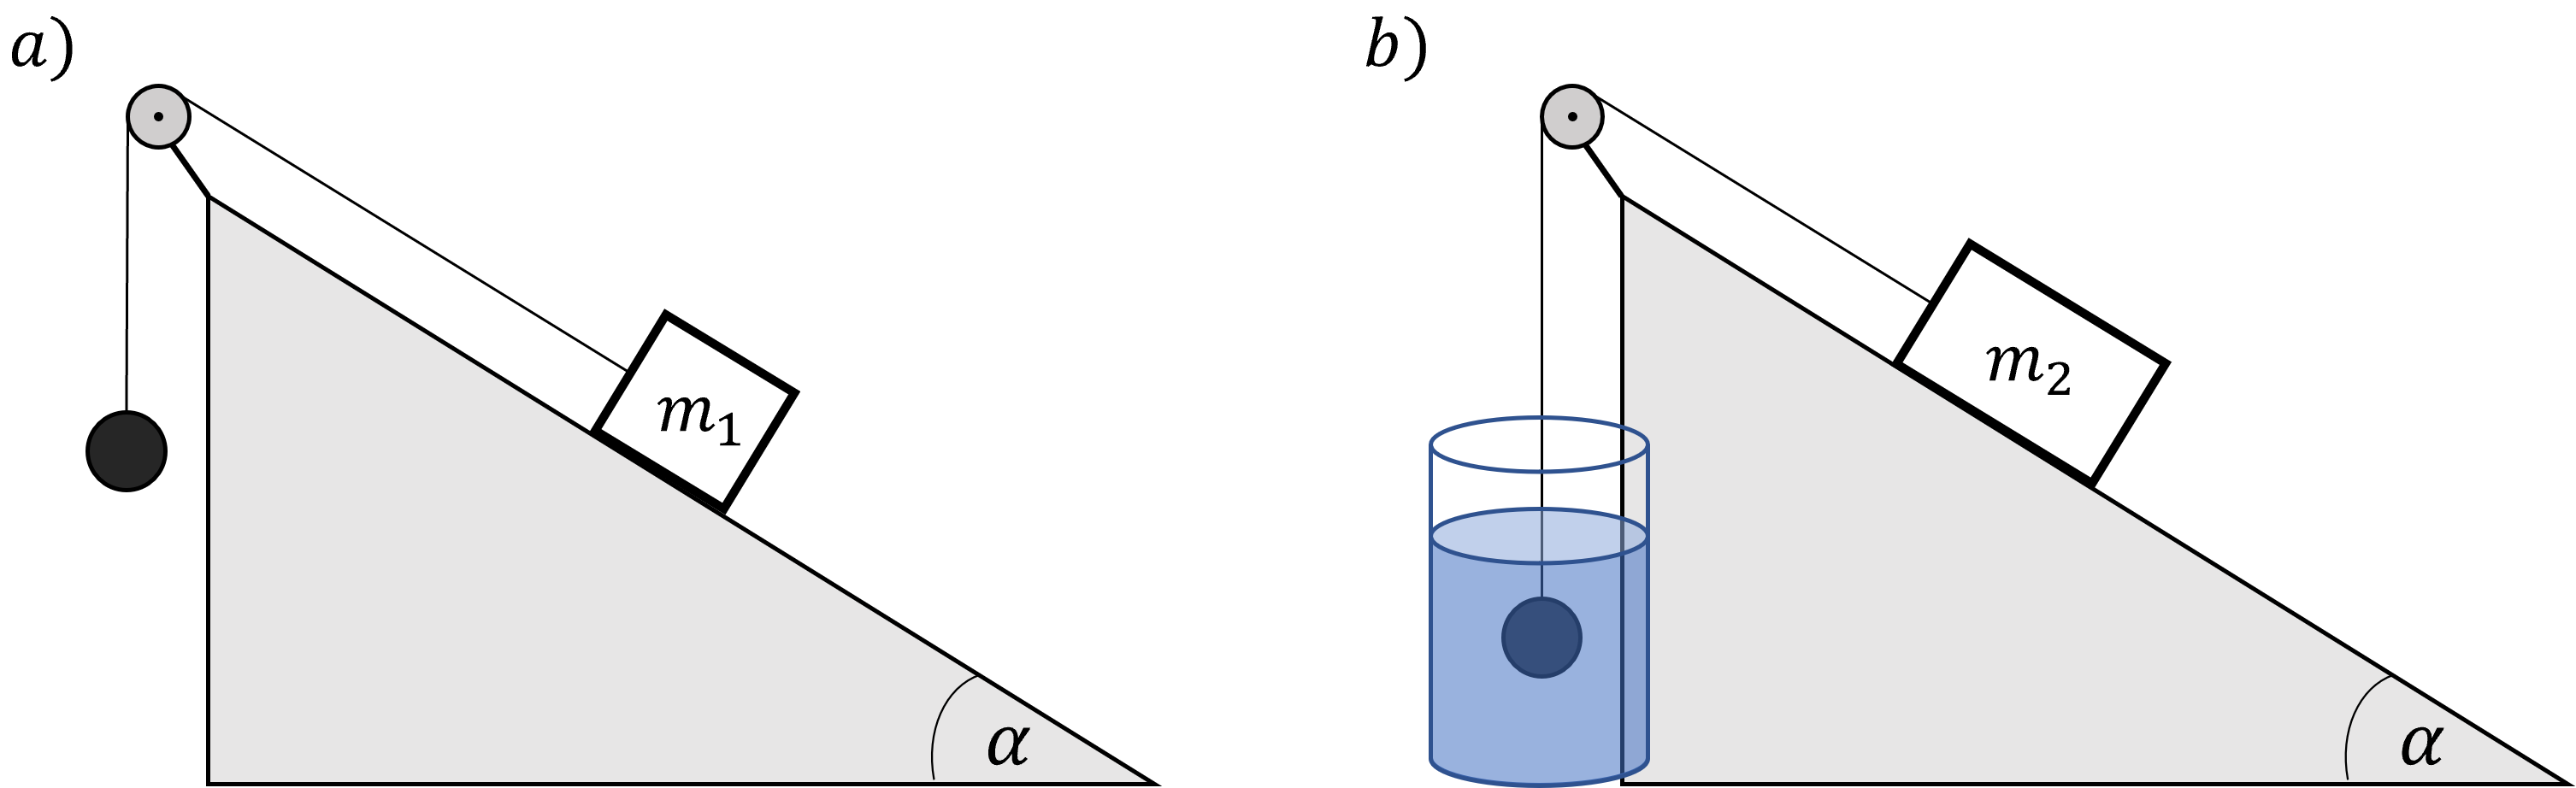
\includegraphics[width=0.7\linewidth]{2022-1/img/auxCrec2/esfera.png}
    \end{figure}

\item Una partícula de masa $m$, que se encuentra en una superficie inclinada, está atada al extremo de una cuerda de largo $L$, inicialmente en reposo y en una cierta posición caracterizada por el ángulo $\beta$ como se muestra la Figura 2. Considere que a partir de un ángulo $\theta$ la superficie presenta roce (tramo C-D en la Figura). Además, en el punto más bajo (B) hay un dispositivo que le entrega a la partícula $\Delta E$ de energía.

Determine el $\Delta E$ mínimo tal que la partícula logre llegar al punto más alto manteniendo la cuerda tensa.

\item Considere un bloque de masa $m$ sostenido por dos resortes de largo natural nulo y con constantes elásticas $k_1$ y $k_2$ como se muestra en la figura. Una vez que el sistema alcanza el equilibrio, se lanza un proyectil de masa $m$ a una velocidad $v$. Si el proyectil y el bloque terminan viajando juntos, determine:

    \begin{enumerate}
        \item La elongación de cada resorte en el equilibrio (pre-colisión).
        
        \item La máxima elongación de cada resorte tras la colisión. Considere que el sistema proyectil-bloque se mueve horizontalmente.
    \end{enumerate}
    
    \textbf{\textit{Hint}}: Encuentre la relación geométrica entre las elongaciones de los resortes pre-colisión y una vez que el sistema ha alcanzado la máxima elongación. Note los triángulos rectángulos que se forman.
    
\begin{figure}[H]
        \centering
        \begin{subfigure}[t]{0.45\textwidth}
            \centering
            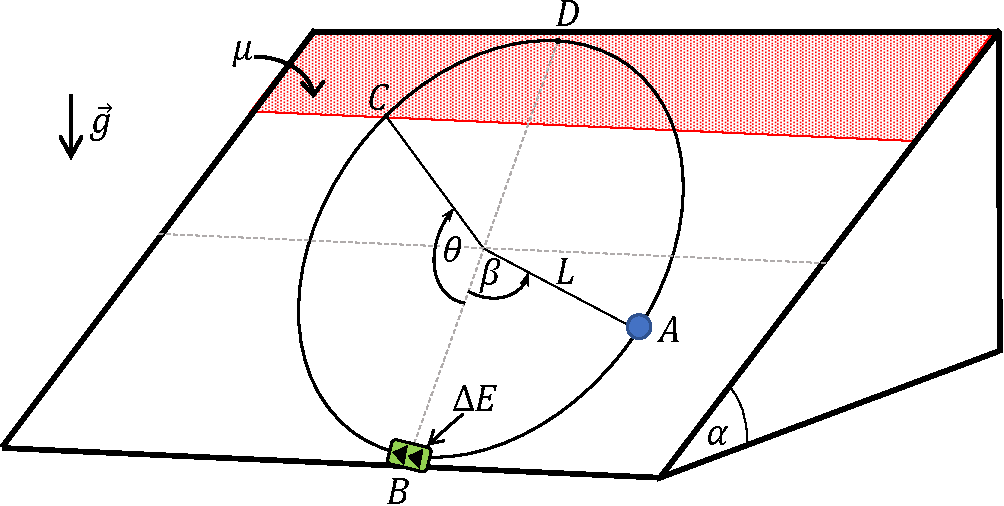
\includegraphics[width=0.9\linewidth]{2022-1/img/auxCrec2/p2c2.pdf}
            \caption{Problema 2.}
        \end{subfigure}
        \hspace{1em}
        \begin{subfigure}[t]{0.40\textwidth}
            \centering
            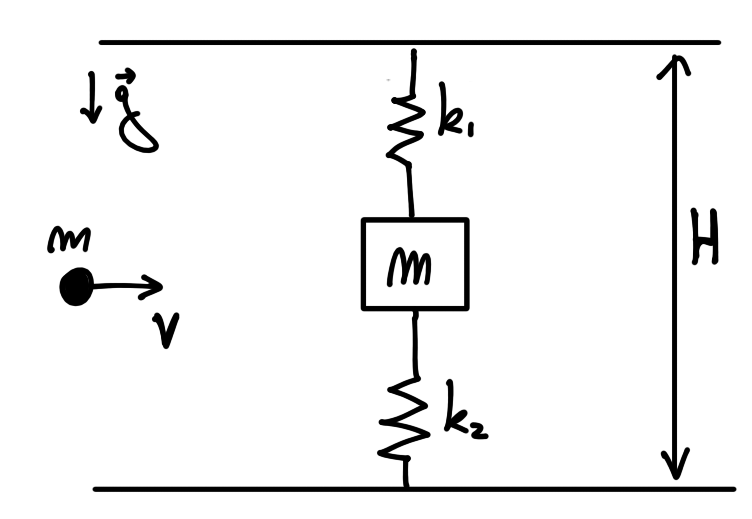
\includegraphics[width=0.8\linewidth]{2022-1/img/auxCrec2/p3c2.png}
            \caption{Problema 3}
        \end{subfigure}
\end{figure}

\item Una varilla de largo $L$ y densidad $\rho_1$ flota en un líquido de densidad $\rho_0$ $\left(\rho_0 > \rho_1\right)$. Un extremo de la varilla se amarra a un hilo a una profundidad $h$.

\begin{multicols}{2}
    \begin{enumerate}
        \item Determine el ángulo $\alpha$
        \item ¿Cuál es el mínimo valor de h para el cual la varilla se mantiene en posición vertical?
        \item Si $A$ es la sección transversal de la varilla, encuentre la tensión del hilo
    \end{enumerate}
    
    \columnbreak
    
    \begin{figure}[H]
        \centering
        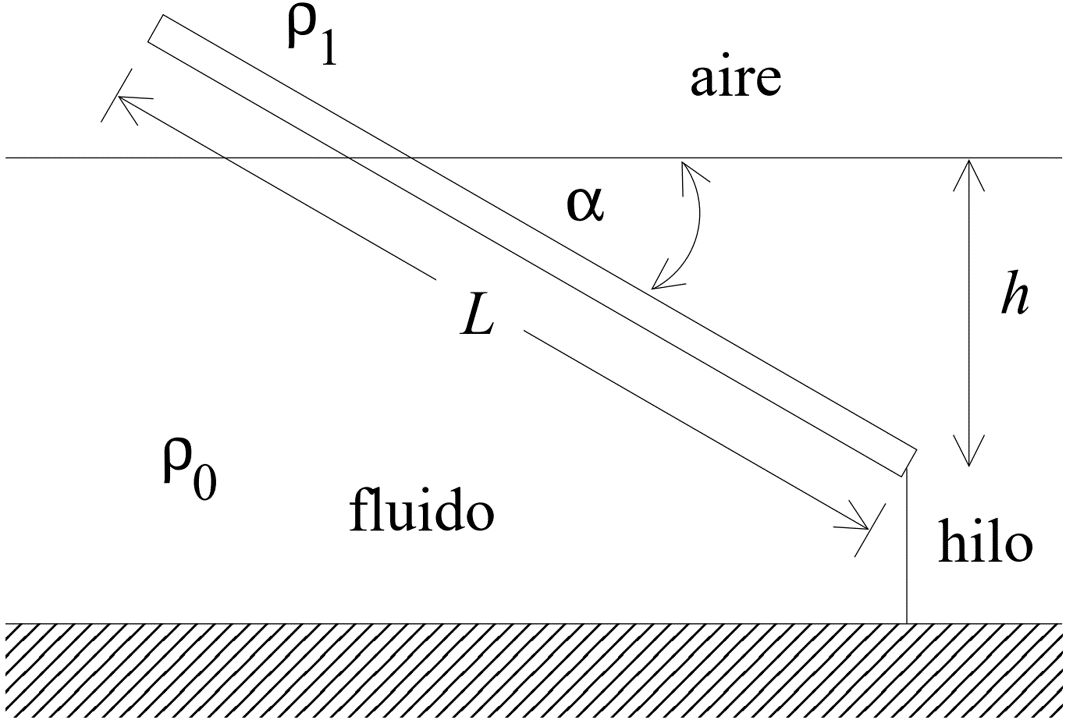
\includegraphics[width=0.55\linewidth]{2021-2/img/aux13/p1.png}
    \end{figure}
\end{multicols}

\item Un tubo en U abierto en ambos extremos se llena parcialmente con mercurio. A continuación se vierten $m=\SI{100}{\g}$ de agua en el brazo derecho, como se muestra en la figura. Si el brazo izquierdo del tubo tiene un área de sección transversal $A_1=\SI{10}{\cm^2}$ y el brazo derecho tiene un área de sección transversal $A_2=\SI{5}{\cm^2}$, determine:
\begin{multicols}{2}
    \begin{enumerate}
        \item La longitud de la columna de agua en el brazo derecho del tubo
        \item Si la densidad del mercurio es $\rho_{Hg}~=~\SI{13.6}{\g/\cm^3}$, ¿qué distancia h se eleva el mercurio en el brazo izquierdo?
    \end{enumerate}
    \columnbreak
    \begin{figure}[H]
        \centering
        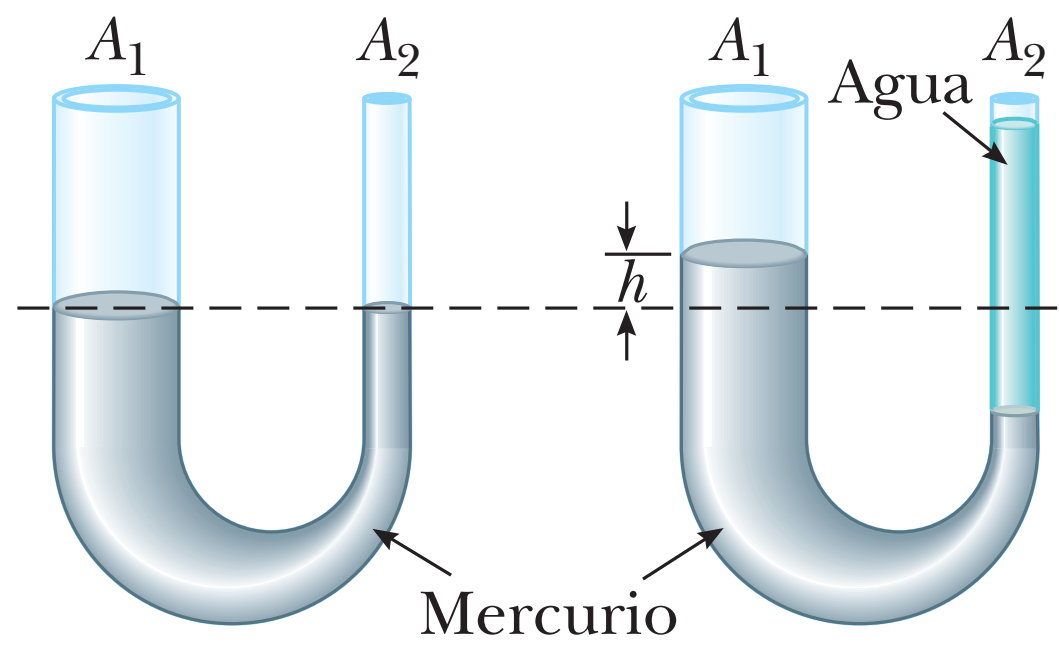
\includegraphics[width=0.5\linewidth]{2021-2/img/aux13/p2.png}
    \end{figure}
\end{multicols}

\item
\begin{multicols}{2}
    Dos globos esféricos inflados con un gas incompresible de densidad $\rho_g$, ambos de radio $R$, se unen mediante una cuerda de longitud $L$. Los dos globos se mantienen bajo el agua con el punto medio de la cuerda fijo al fondo. Calcular la fuerza de contacto entre los globos.
    
    \columnbreak
    
    \begin{figure}[H]
        \centering
        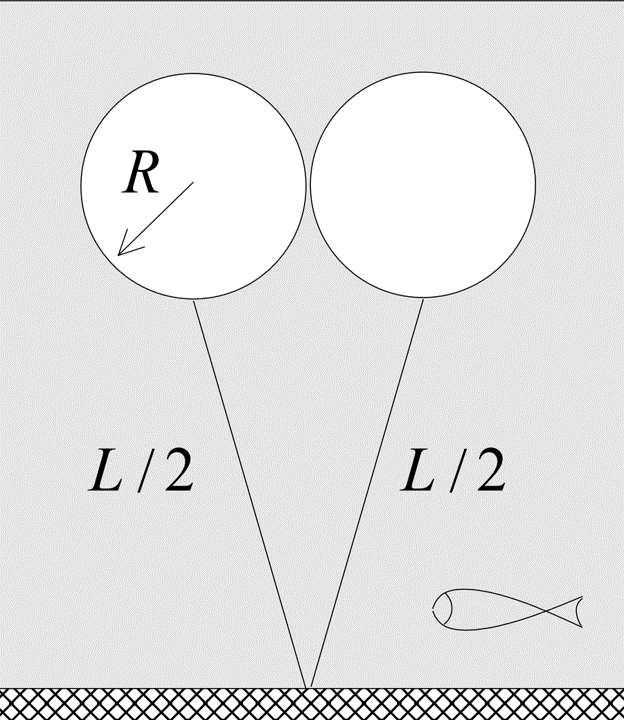
\includegraphics[height=0.4\linewidth]{2021-2/img/aux14/globos.png}
    \end{figure}
\end{multicols}


\item
\begin{multicols}{2}
    Un cubo de madera de longitud $H$ flota en la interfaz entre aceite y agua con su superficie inferior a una distancia $h$ de la interfaz. Si la densidad del aceite es $\rho_{a}$ y la densidad del agua es $\rho_{w}$
    
        \begin{enumerate}
            \item Determine la presión manométrica en la superficie superior e inferior del bloque
            \item Determine la densidad y la masa del bloque 
        \end{enumerate}
    
    \columnbreak
    
    \begin{figure}[H]
        \centering
        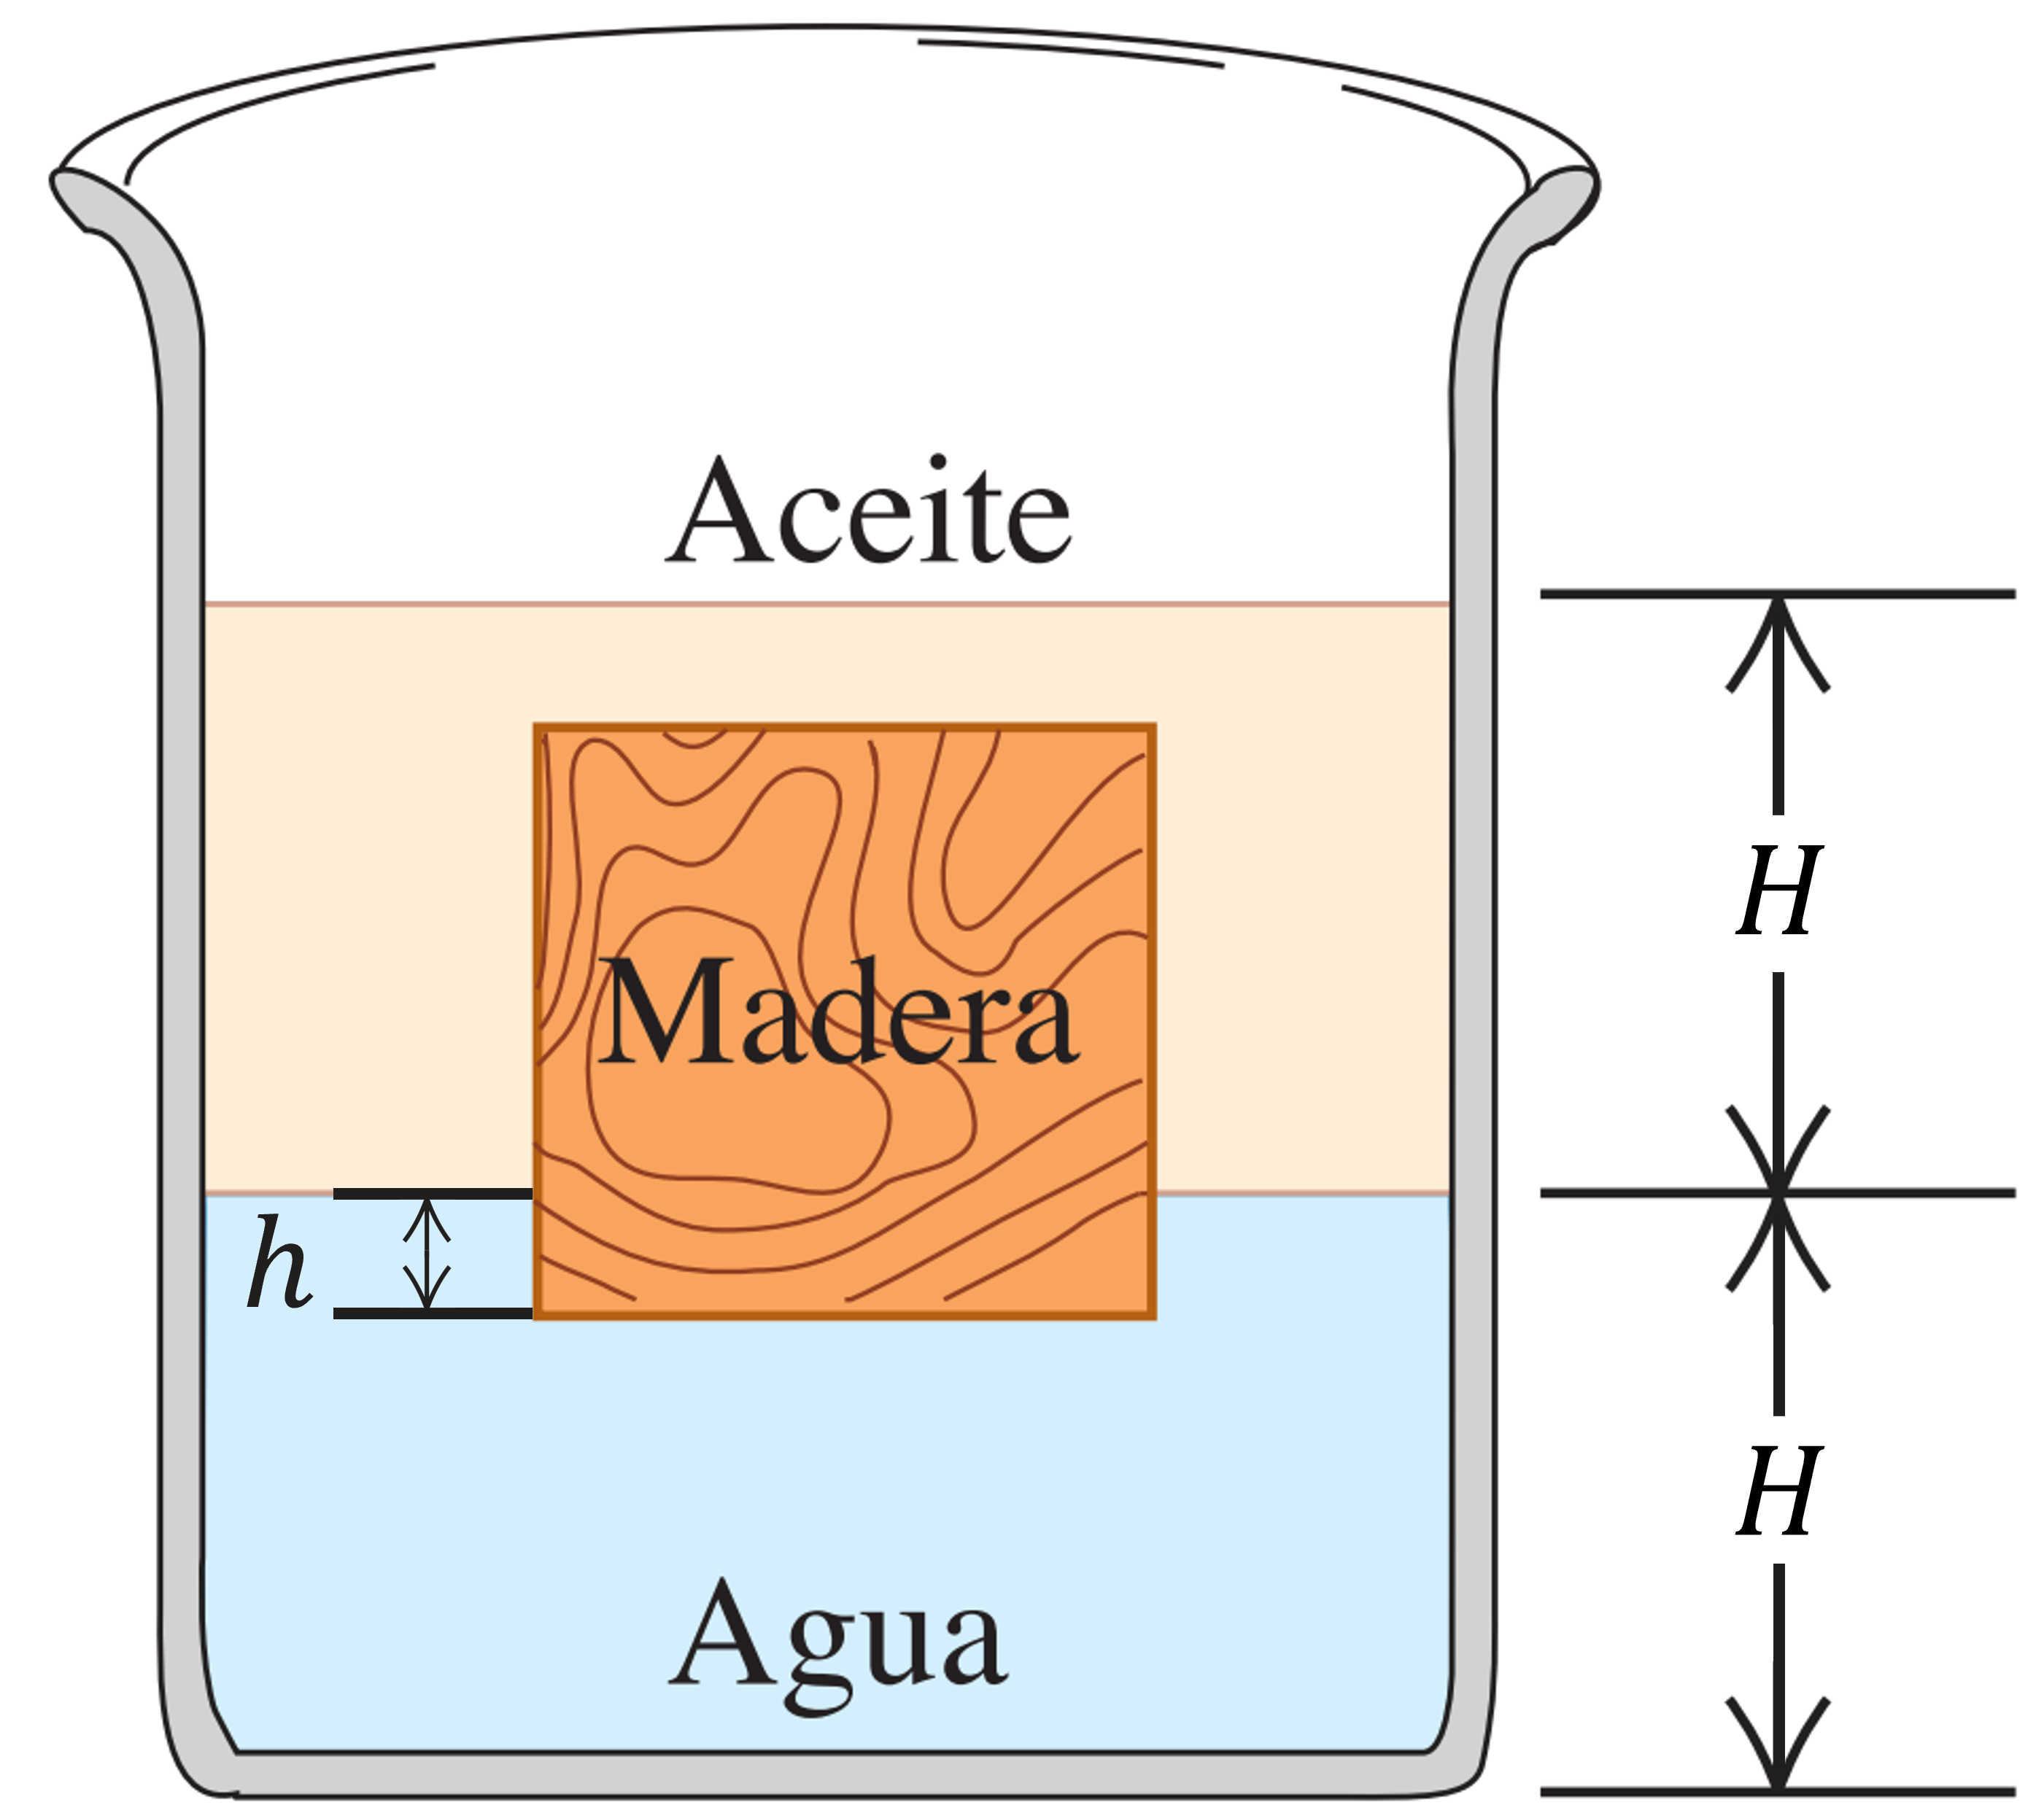
\includegraphics[width=0.45\linewidth]{2021-2/img/aux14/cubo-madera.png}
    \end{figure}
\end{multicols}

% Para imágenes vectoriales -> el texto tiene que estar en LaTeX
% \begin{figure}[htbp]
%   \centering
%   \svgpath{../Imagenes/ejercicios}  -> .. irse pa'trás 
%   \includesvg{ej5.svg}
% \end{figure}

\end{enumerate}
\end{document}
